% Área sob a curva: integral definida
% Feito para o ÉguaTeX (eguatex.com.br). Uso livre (CC0 1.0).
%
% Compile e pronto: sai só a figura, em PDF.
% Para pôr no seu trabalho, use o PDF com \includegraphics ou copie
% o bloco tikzpicture para dentro de uma figure.
\documentclass[tikz,border=4pt]{standalone}
\usepackage[T1]{fontenc}
\usepackage{lmodern}
\usepackage{amsmath}

\colorlet{corArea}{blue!55!white}
\colorlet{corCurva}{blue!70!black}

\begin{document}
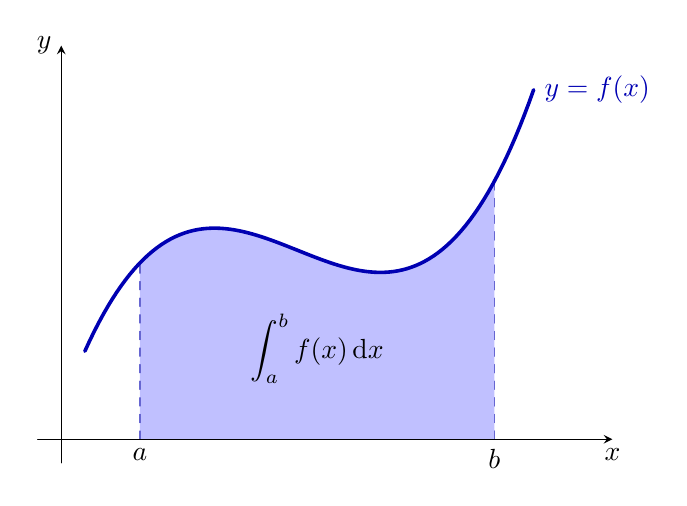
\begin{tikzpicture}[line cap=round, line join=round, >=stealth,
  % Mude a função aqui. Use valores positivos no intervalo do desenho.
  declare function={f(\x) = 0.12*(\x-3)^3 - 0.4*(\x-3) + 2.4;}]

% Mude estes números e o desenho e os rótulos acompanham.
\def\a{1}     % começo do intervalo
\def\b{5.5}   % fim do intervalo
\def\xmax{7}  % até onde vai o eixo x
\def\ymax{5}  % até onde vai o eixo y
\def\xfim{6}  % até onde a curva vai

% área sombreada entre a curva e o eixo x
\fill[corArea, opacity=0.45] (\a,0) -- plot[domain=\a:\b, samples=80] (\x,{f(\x)}) -- (\b,0) -- cycle;
\draw[corCurva!60, dashed] (\a,0) -- (\a,{f(\a)});
\draw[corCurva!60, dashed] (\b,0) -- (\b,{f(\b)});

% eixos
\draw[->] (-0.3,0) -- (\xmax,0) node[below] {$x$};
\draw[->] (0,-0.3) -- (0,\ymax) node[left] {$y$};
\node[below] at (\a,0) {$a$};
\node[below] at (\b,0) {$b$};

% curva
\draw[corCurva, line width=1.3pt] plot[domain=0.3:\xfim, samples=100] (\x,{f(\x)})
  node[right] {$y=f(x)$};

% rótulo da área
\node at ({(\a+\b)/2},{f((\a+\b)/2)/2}) {$\displaystyle\int_a^b f(x)\,\mathrm{d}x$};
\end{tikzpicture}
\end{document}
